\section{LaTeX}
\label{sec:latex}

\noindent There are several text editors that include tools for working with LaTeX. I don't really like any of them. Emacs has a natural ``latex-mode'' that does some syntax highlighting---and there's a lot you can do the integrate LaTeX with Emacs (see, for example, Nick Higham's blog: \url{https://nickhigham.wordpress.com/category/latex/}). However, I don't use any of it. I just use Emacs to create~.tex documents. 

I compile a completed~.tex file with a Makefile that executes LaTeX commands. From the command line, just type \texttt{make}. My Makefile's contain two ways to compile: (i) with \texttt{latex} and (ii) with \texttt{pdflatex}. The latter is preferred, but some journal templates need to use the former (for some reason). 

Here are some sample environments I use regularly in papers. See Algorithm \ref{alg:0} and Figure \ref{fig:0} with Subfigures \ref{fig:sub0} and \ref{fig:sub1}. 

\begin{algorithm}
Given some stuff, do the following:
\begin{enumerate}
\itemsep0em
\item Step 1
\item Step 2
\end{enumerate}
\caption{My favorite algorithm}
\label{alg:0}
\end{algorithm}

\begin{figure}[!h]
\centering
\subfloat[Label 1]{
\label{fig:sub0}
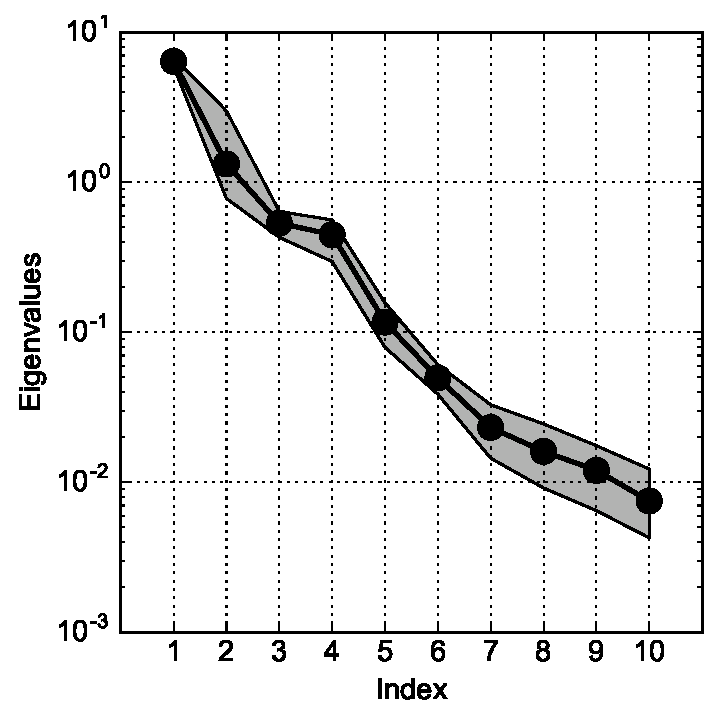
\includegraphics[width=0.42\textwidth]{figs/evals_drag.eps}%
}
\hfil
\subfloat[Label 2]{
\label{fig:sub1}
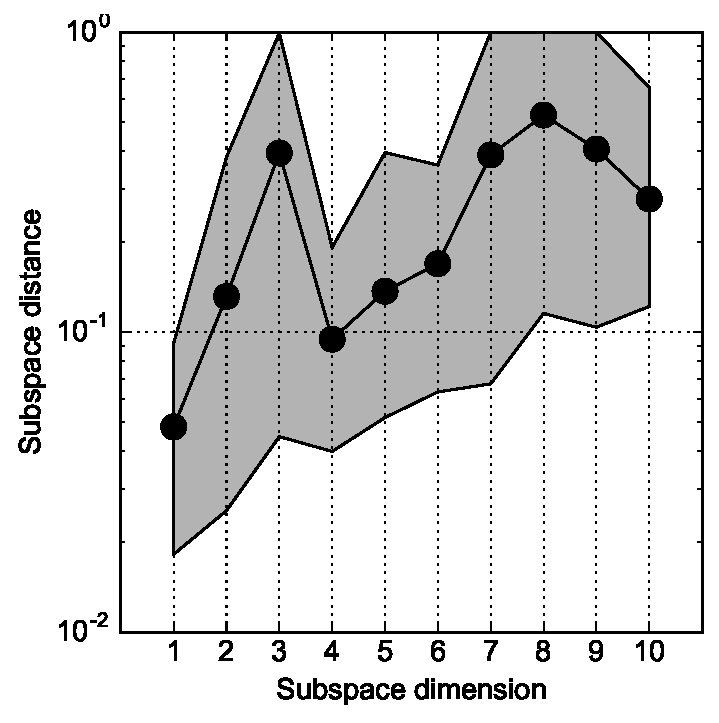
\includegraphics[width=0.42\textwidth]{figs/subspace_drag.eps}%
}
\caption{And this is where you put the caption}
\label{fig:0}
\end{figure}

I usually make figures in the code directory and manually move them to the \texttt{paper\_v0/figs} directory. That way, if I change the figure in the code because I'm playing around, then it doesn't immediately change the paper figure.
